In questa sezione verrà illustrato l'ambiente di lavoro che sarà utilizzato durante lo sviluppo del progetto \PROGETTO.\\

\subsection{Protocollo per la gestione del progetto}

\subsubsection{Creazione e gestione dei ticket}

I \gls{ticket} vengono creati e gestiti quasi tutti dal \textit{Responsabile di Progetto}.
Qualora il \textit{Verificatore} trovasse imprecisioni o errori durante la verifica, avrà la possibilità di creare dei \gls{ticket} per segnalare suddetti errori.
Ogni \gls{ticket} può essere assegnato ad uno o più membri del gruppo a seconda della complessità del lavoro e della disponibilità dei membri del gruppo.
Per creare un nuovo \gls{ticket} bisogna:

\begin{itemize}
	\item Posizionarsi alla voce Issue;
	\item Premere "New issue";
	\item Compilare i campi richiesti:
	\begin{itemize}
		\item \textbf{Titolo e commenti:} titolo descrittivo con una descrizione del nuovo \gls{ticket};
		\item \textbf{Labels:} dovranno avere due caratteristiche fondamentali e cioè la tipologia di \gls{ticket} assegnato(modifica, verifica, richiesta approvazione) e la priorità assegnata(alta, media, bassa);
		\item \textbf{\gls{Milestone}:} la \gls{milestone} a cui è associato il \gls{ticket};
		\item \textbf{Assignee:} a chi viene assegnato il \gls{ticket}.
	\end{itemize}
\end{itemize}
\begin{figure}[h]
	\centering
	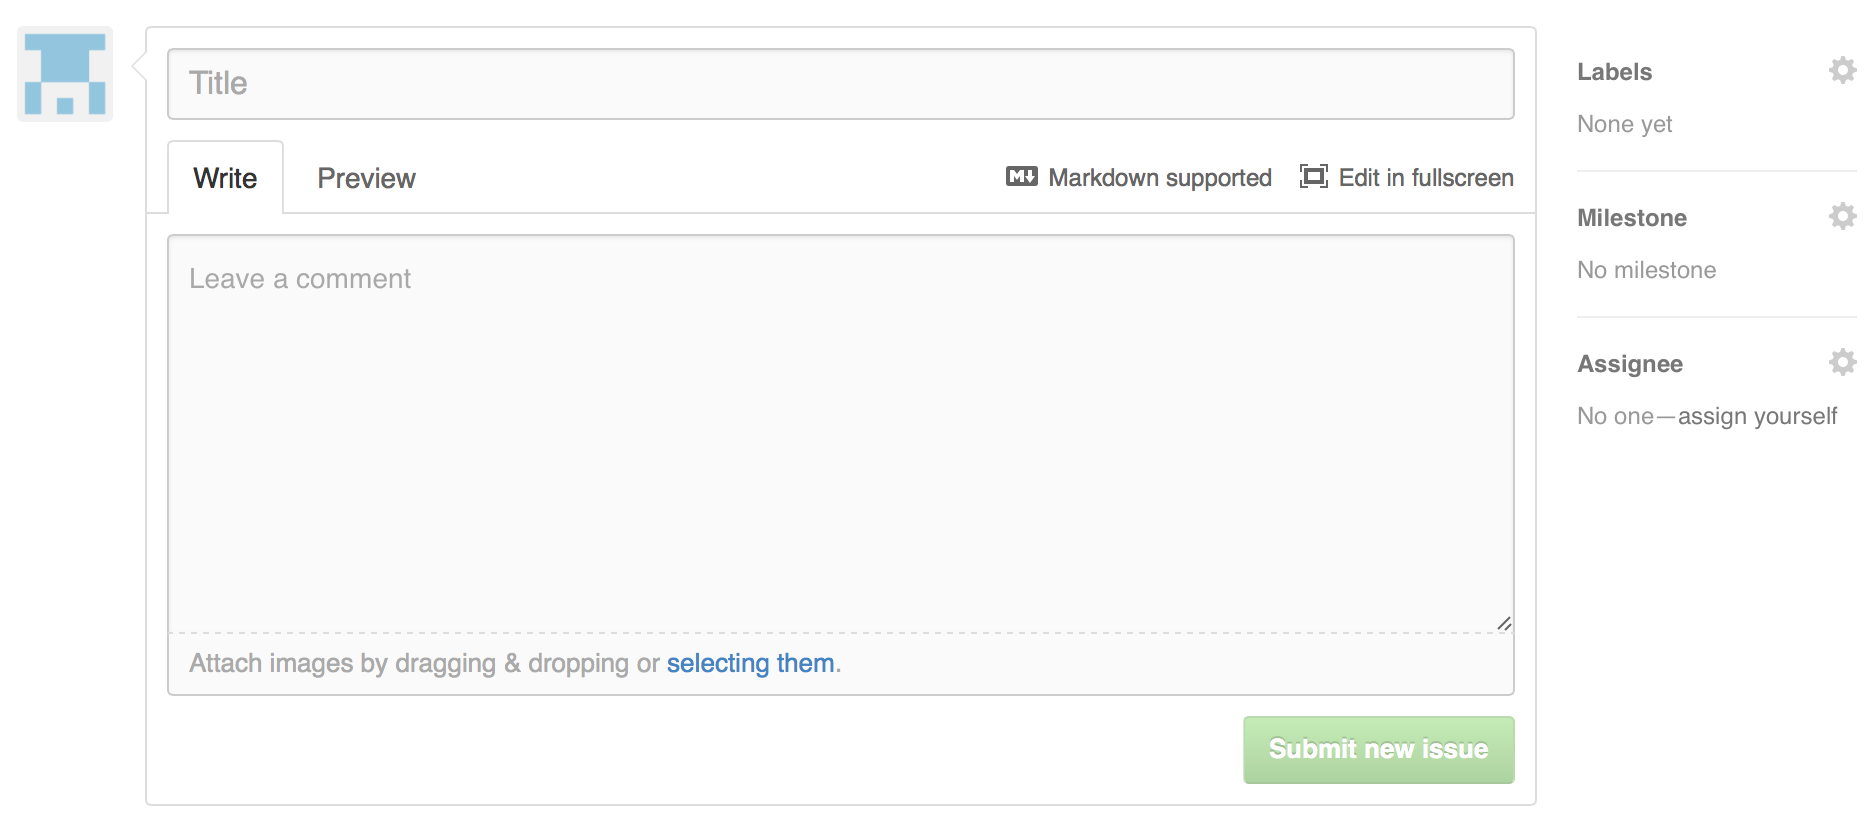
\includegraphics[width=0.7\linewidth]{img/ticket}
	\caption[Creazione ticket]{Creazione ticket}
	\label{fig:ticket}
\end{figure}

\newpage
\subsubsection{Creazione delle milestone}

Il \textit{Responsabile di Progetto} ha il compito della creazione di una \gls{milestone} in occasione di ogni revisione al quale il gruppo \GRUPPO\ ha intenzione di partecipare, più altre \gls{milestone} qualora il \textit{Responsabile di Progetto} lo ritenga necessario.

Per creare una nuova \gls{milestone} bisogna:

\begin{itemize}
	\item Posizionarsi alla voce \gls{Milestone};
	\item Premere "New \gls{milestone}";
	\item Compilare i campi richiesti:
	\begin{itemize}
		\item \textbf{Titolo;}
		\item \textbf{Descrizione;}
		\item \textbf{Data.}
	\end{itemize}
\end{itemize}
\begin{figure}[h]
	\centering
	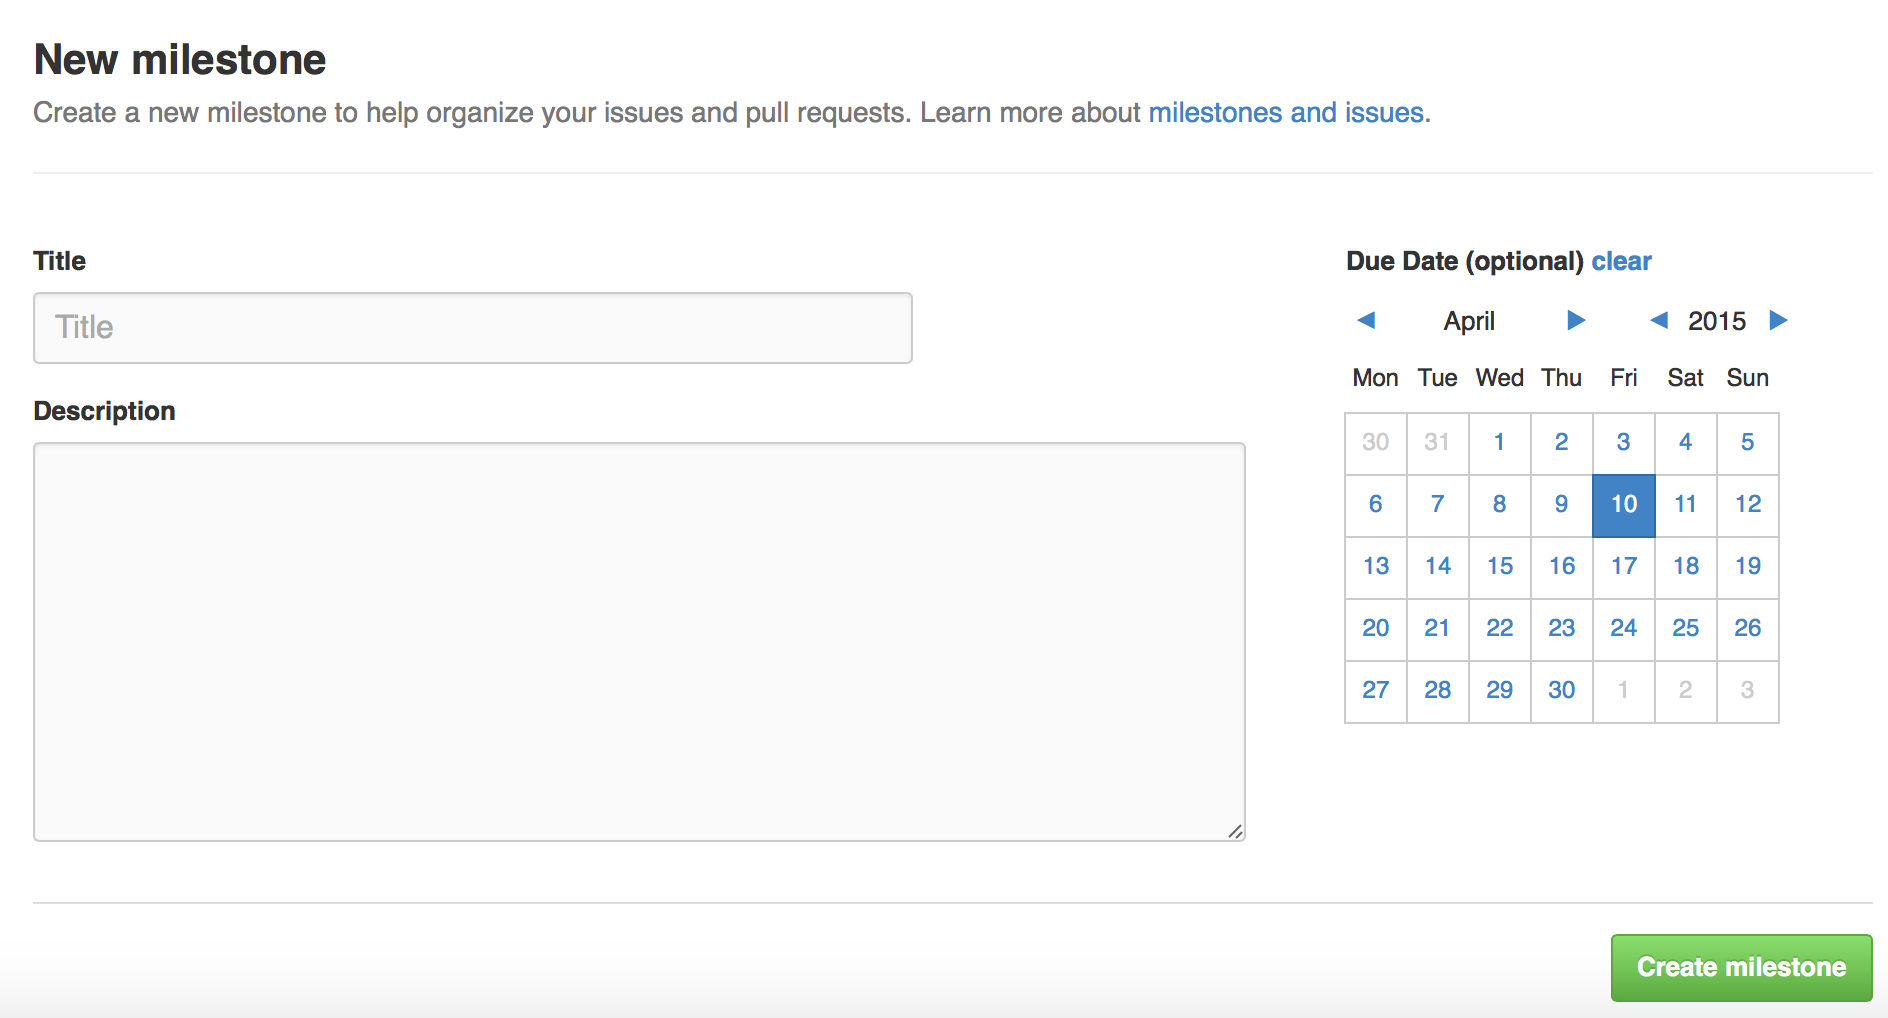
\includegraphics[width=0.7\linewidth]{img/milestone}
	\caption[Creazione milestone]{Creazione milestone}
	\label{fig:milestone}
\end{figure}

\subsubsection{Esecuzione dei compiti}

Ogni membro del gruppo è tenuto a visionare regolarmente la presenza di \gls{ticket} a lui assegnati e segnalarne la presa in consegna.
Una volta che un membro porta a termine un \gls{ticket} deve modificarne lo stato per segnalare il termine del lavoro.
Se un \gls{ticket} non ha avuto i risultati attesi il \textit{Responsabile di Progetto} può riaprirlo ed eventualmente assegnare altri membri al lavoro.

\subsubsection{Chiusura della milestone}

Una volta raggiunta la scadenza il \textit{Responsabile di Progetto} deve chiudere la \gls{milestone} ed eventualmente aprirne un'altra per poi ricominciare tutto il protocollo da capo.




\subsection{Sistema operativo}

Il sistema operativo utilizzato è lasciato a discrezione di ogni membro del gruppo. Questa scelta è dovuta principalmente al fatto che il progetto dovrà supportare più piattaforme.
I membri del gruppo utilizzeranno i seguenti sistemi operativi:

\begin{itemize}
	\item \gls{Windows} 7 64 bit;
	\item \gls{Windows} 8.1;
	\item \gls{Ubuntu} 14.10;
	\item Mac OS 10.10.2.
\end{itemize}

\subsection{Coordinamento}

Il coordinamento del gruppo avviene tramite:
\begin{itemize}
	\item \gls{Google Drive};
	\item \gls{Google Calendar};	
	\item \gls{Repository} \gls{Git}.
\end{itemize}

\subsubsection{Google Drive}

Abbiamo scelto di utilizzare questo \gls{servizio cloud} per condividere tutti i documenti che non necessitano di \gls{versionamento} e vengono utilizzati frequentemente da parte dei membri del gruppo. 
È un servizio molto semplice e accessibile direttamente da \gls{browser} che permette di lavorare su documenti creati con \gls{Google Docs}.

\subsubsection{Google Calendar}
\gls{Google Calendar} viene utilizzato per la gestione delle risorse umane e per tenere traccia degli eventi importanti. È stato creato un calendario condiviso con tutti i membri del gruppo in modo da conoscere le date in cui una persona è assente o non reperibile e le date rilevanti per il gruppo.\\
Inoltre è possibile modificare la gestione delle notifiche per un evento o più eventi in modo che venga inviata automaticamente una email a tutti i membri del gruppo. In questo caso il preavviso deve essere di almeno un giorno.

\subsubsection{Repository Git}

Nonostante siano disponibili molti \gls{repository} (\gls{Git}, \gls{Mercurial}, \gls{SVN}) è stato scelto di utilizzare \gls{Git} in quanto il servizio soddisfa pienamente le necessità di \gls{hosting} e \gls{versionamento} necessarie per lo sviluppo di questo progetto, inoltre diversi membri del gruppo avevano già usato tale servizio. Esso permette di lavorare senza una connessione attiva a internet e da la possibilità di ignorare alcune estensioni specificate in un file chiamato .gitignore\footnote{File globale di \gls{Git} che contiene una lista di regole per ignorare i file.}.\\ Per i membri del gruppo che desiderano utilizzare un client, si consigliano i seguenti:
\begin{itemize}
	\item \textbf{SourceTree};
	\item \textbf{\gls{GitHub}};
\end{itemize}
Per maggiori dettagli si rimanda alla sezione \ref{repository}.

\newpage
\paragraph{Utilizzo del servizio}
È necessario eseguire le operazioni di sincronizzazione all'inizio e alla fine di ogni sessione di lavoro. \\
In particolare ad ogni sessione di lavoro andranno eseguite le seguenti operazioni:
\begin{itemize}
	\item \textbf{Pull}: scaricare la versione più aggiornata del progetto per poterci poi lavorare offline;
	\item \textbf{Add}: aggiungere i file ad uno specifico elenco generando una proposta di modifica;
	\item \textbf{Commit}: validare le proposte fatte in precedenza;
	\item \textbf{Push}: serve a pubblicare i risultati online, sulla piattaforma di sviluppo;
	\item \textbf{Merge}: permette di fondere un \gls{branch} con il \gls{repository} padre, così da implementare le modifiche apportate ai file e alle cartelle originarie.
\end{itemize}
\begin{figure}[h]
\centering
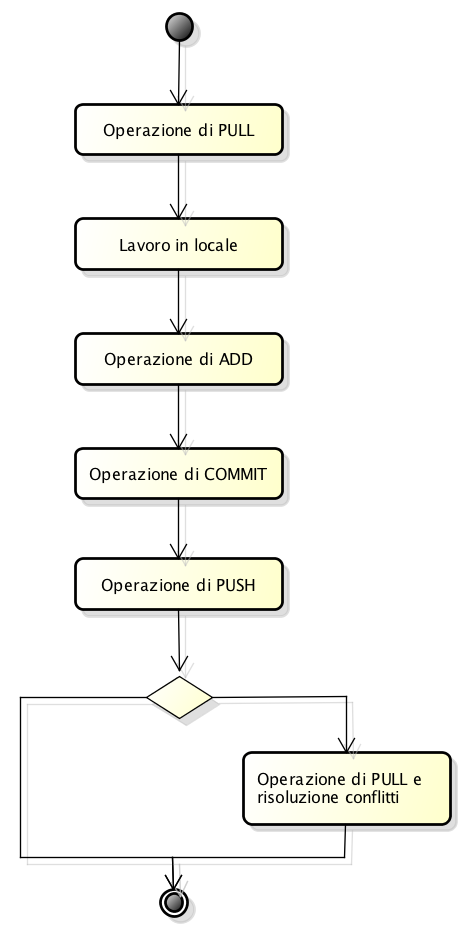
\includegraphics[width=0.5\linewidth]{img/proceduraRepository}
\caption[Procedura per l'utilizzo del Repository]{Procedura per l'utilizzo del Repository}
\label{fig:proceduraRepository}
\end{figure}

\noindent È vietato utilizzare "git add *" per evitare di includere file nascosti. Tutti i membri del gruppo dovono essere consapevoli dell'esatto contenuto dei file. Ogni commit deve essere corredato di un messaggio che descriva in modo \gls{conciso} il lavoro svolto.

\newpage
\subsection{Ambiente documentale}

\subsubsection{Stesura documenti}

Per la stesura dei documenti verrà utilizzato il \gls{linguaggio di markup} \LaTeX.
Come editor è consigliato TeXstudio\footnote{\url{http://texstudio.sourceforge.net}}, il quale è disponibile per tutti i principali sistemi operativi.

\subsubsection{Script}

Per facilitare la stesura dei documenti sono stati creati alcuni script:

\begin{itemize}
	\item Generazione di tutti i documenti PDF: con il comando "make all" verranno generati tutti i PDF dei documenti contenuti nella directory corrente;
	%\item Controllo ortografico: con il comando make aspell verrà invocato il programma aspell su tutti i documenti della directory corrente;
	%\item Eliminazione file errati o vecchi: con il comando make clean verranno eliminatati i file generati da compilazioni vecchio o file non necessari della directory corrente;
	\item Evidenziare glossario: con il comando "java glossary" verrà eseguito uno script che selezionerà nei documenti della directory corrente le parole contenute nella versione più recente del glossario e le evidenzierà con il simbolo "\G".

\end{itemize}

\subsubsection{Pianificazione delle attività}
Per pianificare le attività e la gestione del progetto e delle risorse umane si è scelto di usare \gls{GanttProject}\footnote{\url{http://www.ganttproject.biz}}.

\subsection{Ambiente di sviluppo}
Secondo il decreto legislativo n.81, ogni 120(centoventi) minuti passati in maniera continuativa davanti al computer ogni membro deve fare almeno quindici minuti interruzione.\footnote{\url{http://www.pmi.it/impresa/normativa/news/51788/dipendenti-al-pc-obblighi-di-legge-per-i-datori-di-lavoro.html}}

\subsection{Diagrammi UML}

Per la realizzazione dei diagrammi \gls{UML} è stato scelto \gls{Astah} Professional Edition\footnote{\url{http://astah.net/download}}.
È possibile ricevere gratuitamente la licenza della versione professional inviando una richiesta al sito \url{http://astah.net/student-license-request}.


